\documentclass[onecolumn, draftclsnofoot,10pt, compsoc]{IEEEtran}
\usepackage{graphicx}
\usepackage{url}
\usepackage{setspace}
\usepackage{listings}
\usepackage{xcolor}
\usepackage{caption}
\usepackage{subcaption}
\usepackage{float}
\usepackage{longtable}
\usepackage{pdfpages}

\graphicspath{ {./img/} }

\newcommand{\subparagraph}{}

\newcommand{\fakesection}[1]{%
  \par\refstepcounter{section}% Increase section counter
  \sectionmark{#1}% Add section mark (header)
  \addcontentsline{toc}{section}{\protect\numberline{\thesection}#1}% Add section to ToC
  % Add more content here, if needed.
}

\usepackage[explicit]{titlesec}

\usepackage{pgfgantt}
\definecolor{grey}{rgb}{0.57, 0.64, 0.69}

\usepackage{geometry}
\geometry{textheight=9.5in, textwidth=7in}

% Listings settings for swift taken from chriseidhof GitHub
\lstdefinelanguage{swift}
{
  morekeywords={
    func,if,then,else,for,in,while,do,switch,case,default,where,break,continue,fallthrough,return,
    typealias,struct,class,enum,protocol,var,func,let,get,set,willSet,didSet,inout,init,deinit,extension,
    subscript,prefix,operator,infix,postfix,precedence,associativity,left,right,none,convenience,dynamic,
    final,lazy,mutating,nonmutating,optional,override,required,static,unowned,safe,weak,internal,
    private,public,is,as,self,unsafe,dynamicType,true,false,nil,Type,Protocol,
  },
  morecomment=[l]{//}, % l is for line comment
  morecomment=[s]{/*}{*/}, % s is for start and end delimiter
  morestring=[b]" % defines that strings are enclosed in double quotes
}

\definecolor{keyword}{HTML}{BA2CA3}
\definecolor{string}{HTML}{D12F1B}
\definecolor{comment}{HTML}{008400}

\lstset{
  language=swift,
  basicstyle=\ttfamily,
  showstringspaces=false, % lets spaces in strings appear as real spaces
  columns=fixed,
  keepspaces=true,
  keywordstyle=\color{keyword},
  stringstyle=\color{string},
  commentstyle=\color{comment},
}

% From chriseidhof on GitHub

\definecolor{NASAred}{RGB}{252,61,33}
\definecolor{NASAblue}{RGB}{11,61,145}

\definecolor{OSUorange}{RGB}{220,68,5}

\definecolor{myblue}{HTML}{1563e0}
\definecolor{mygrey}{HTML}{ADBED8}
\definecolor{mydarkgrey}{HTML}{3d434c}

% 1. Fill in these details
\def \CapstoneTeamName{Manovacumeter Team}
\def \CapstoneTeamNumber{ 20}
\def \GroupMemberOne{Cade Raichart}
\def \GroupMemberTwo{Daniel Kato}
\def \GroupMemberThree{Nathan Shepherd}
\def \CapstoneProjectName{ISS Barometer App }
\def \CapstoneSponsorCompany{NASA}
\def \CapstoneSponsorPerson{Don Pettit}

% 2. Uncomment the appropriate line below so that the document type works
\def \DocType{Final Report}

\newcommand{\NameSigPair}[1]{\par
\makebox[2.75in][r]{#1} \hfil 	\makebox[3.25in]{\makebox[2.25in]{\hrulefill} \hfill		\makebox[.75in]{\hrulefill}}
\par\vspace{-12pt} \textit{\tiny\noindent
\makebox[2.75in]{} \hfil		\makebox[3.25in]{\makebox[2.25in][r]{Signature} \hfill	\makebox[.75in][r]{Date}}}}
% 3. If the document is not to be signed, uncomment the RENEWcommand below
%\renewcommand{\NameSigPair}[1]{#1}

%%%%%%%%%%%%%%%%%%%%%%%%%%%%%%%%%%%%%%%
\begin{document}
\begin{titlepage}
    \pagenumbering{gobble}
    \begin{singlespace}
    	\includegraphics[height=4cm]{coe_v_spot1}
        \hfill
        % 4. If you have a logo, use this includegraphics command to put it on the coversheet.
        %
\includegraphics[height=4cm]{NASA}
        \par\vspace{.2in}
        \centering
        \scshape{
            \huge CS Capstone \DocType \par
            {\large\today}\par
            \vspace{.5in}
            \textbf{\Huge\CapstoneProjectName}\par
            \vfill
            {\large Prepared for}\par
            \Huge \CapstoneSponsorCompany\par
            \vspace{5pt}
            {\Large\NameSigPair{\CapstoneSponsorPerson}\par}
            {\large Prepared by }\par
            Group\CapstoneTeamNumber\par
            % 5. comment out the line below this one if you do not wish to name your team
            %\CapstoneTeamName\par
            \vspace{5pt}
            {\Large
                \NameSigPair{\GroupMemberTwo}\par
            }
            \vspace{20pt}
        }
        \begin{abstract}
        % 6. Fill in your abstract

        \end{abstract}
    \end{singlespace}
\end{titlepage}
\newpage
\pagenumbering{arabic}
\tableofcontents
% 7. uncomment this (if applicable). Consider adding a page break.
%\listoffigures
%\listoftables
\clearpage

% 8. now you write!

\section{Introduction to Project}
% (Hint, refer to project proposal and problem statement)
% Who requested it?
% Why was it requested?
% What is its importance?
% Who was/were your client(s)?
% Who are the members of your team?
% What were their roles?
% What was the role of the client(s)? (I.e., did they supervise only, or did they participate in doing development)

N.A.S.A requested this project of us, specifically the astronauts aboard the international space station requested that the project be started. 

The App was wanted to replace the mechanical barometer that are called, Manovacumeters.
These are being used for finding holes that are letting atmospheric pressure out. 
They needed to replace these because they are starting to break, they only have 3 or left. 
The app will also be made to make it so the crew members no longer have to do calculations in their head or on paper, while in emergency situations. 
This is significant for the survival of the team. 
it also is significant because the less time they use for math the more time to find the hole, it helps with resources to because if they can't find the hole then they have to leave the space station meaning they will have to make a whole new mission to bring it back on. 

Don Pettit was our contact from N.A.S.A, he is an astronaut who is a chemical engineer and has spent a year of his life in space on two different six month trips. 
He acted as a supervisor who we would report to and would change how the app looked and worked after each iteration we sent him 

 Nathan Shepherd, Daniel Kato and Cade Raichart are the team members working on the ISS Barometer App. 

\section{Requirements Document}
% include the original document, showing what you thought, at the time, was the project definition with the original Gantt chart

\subsection{Introduction}

\subsubsection{Purpose}
This document will detail the required final product of this project, the \CapstoneProjectName.
The sections will go over the scope of the project, as well as the specific details of it's completion.
This document will also serve as the metrics in which we will be graded at the end of Spring term.
This Requirements Document is meant as a repeatable and detailed description of the problem that we aim to solve, as stated in our Problem Statement.
That goal is to provide an auxiliary barometer to the MANOVACUMETERS aboard the ISS with an iPad app.
The intended audience for this document is the client, NASA and Don Pettit, as well as anyone seeking to repeat this process.
This document will also act as a success metric once this school year is finished, allowing clear decisive evaluation.
Additionally it will provide a detailed agreement between the group and our client, to ensure that we are all on the same page.
This document can be changed throughout the project, but scope changes must be submitted and verified by both teachers and clients.

\subsubsection{Scope}
The \CapstoneProjectName will measure the current pressure of its surroundings using the built in pressure transducer.
The application will display the pressure in mmHg upon starting the app and whenever the 'Record Pressure' button is pressed the current pressure along with a timestamp will be recorded and displayed.
It will also display the current pressure change in $\frac{\Delta t}{\Delta p}$ and include a graph of $\frac{\Delta p}{\Delta t}$ will be displayed with the capability to pinch to zoom and scale the graph.
This graph will have a readout of $\Delta \frac{\Delta p}{\Delta t}$ displayed next to it.
A settings page will be provided that allows the user to choose the plot scale of the graph, orientation of the app, and number of significant digits.
The graph's data will also be exportable as a csv file.
The application will not read remote pressure data.
The \CapstoneProjectName will be used as a tool for astronauts to compute the amount of time they have before they must evacuate the International Space Station.
This application has the benefit of allowing the user to track the change of pressure data more efficiently than taking readings from a manual barometer.

\subsubsection{Definitions, Acronyms, and Abbreviations}
\begin{itemize}
\item[--] csv: A file format readable by Excel and other spread sheet software
\item[--] iOS: The internal operating system of Apple products, specifically iPads
\item[--] iPad: A touch screen tablet device with barometer capabilities
\item[--] ISS: International Space Station
\item[--] MANOVACUMETER: The current mechanical air pressure gauge aboard the ISS
\item[--] mmHg: Millimeters of Mercury, the standard pressure unit
\item[--] NASA: National Aeronautics and Space Administration
\item[--] t-Res: The chart that NASA uses to calculate residual time left on station
%Add any wacko words that are used throughout
\end{itemize}

\subsubsection{References}

\subsubsection{Overview}
This document will follow the IEEE 830-1995 guidelines, in both headings and content.
The following section, Overall Description, will detail the description of our application,
The third section, Specific Requirement, will outline the requirements in user interface, hardware interface, software interface, and communications interface.
Our Gantt chart can be found in section 2.6, Schedule Dependencies, and lays out the rough schedule in terms of dependent features.
It provides a birds-eye view of the schedule and dependencies of this project.
It is subject to change, as more information and insight comes to light.
The final section will describe, in detail, each feature, additionally it will describe second version features.
Second version features are not stretch goals, but instead expected after the first version release in December of 2017, as detailed in our Gantt chart.

\subsection{Overall Description}

\subsubsection{Product Perspectives}
Today in the Apple store there are apps that use the internal barometer and displays earth's atmospheric pressure, one such app is Barometer and Altimeter Pro.
Apps on the market are designed for earth's atmospheric pressure and to help with detection of weather.
The product we are creating will be used for detection atmospheric pressure in space specifically from hull breaches.
To accomplish the requirements the system interfaces will have three pages the display, graph and settings.
The Display will have a big button, with a digital display of atmospheric pressure.
The first page will display the initial pressure, current pressure and the pressure change as sec/mmHG.
Graphs display will have a graph that spans the whole screen, that the user will have the ability to zoom in and out.
 The graph axis will be pressure vs the function of time and our slope will be $\frac{\Delta p}{\Delta t}$.
 The third page, settings page, will control the characteristics and look of the other two pages.
Settings page will contain the option of changing the plot scale, scroll functionality, orientation, decimal point, as well as other units of measure for pressure.
 All displays and pages need to be able to be read fast and easily in low light.
We will need to get the software to use the internal barometer that the iPad Air-2 uses, this will capture our atmospheric pressure for us.
There is no outside interface that the app needs to use to complete the product.
There is a chance that the running graph could impeded on the amount of memory the iPad has, the longer it's on the more data it stores.
This being said the data isn't large and shouldn't be a problem.

\subsubsection{Product Functions}
This application will be released in multiple versions, with the initial version expected to be released by the end of 2017.
As such, the functions are separated into Version 1 requirements and Version 2 requirements.
Additionally, if given time, our team may be able to do accuracy and resistance testing on the iPad devices for low pressure.
This is a stretch goal, and might not be feasible with our current time frame.
The following functions will be detailed in the Specific Requirements subsection, but are presented below for clarity.
\begin{itemize}
\item[V1:] Data Screen with initial pressure, current pressure, start/stop button, time stamp, pressure change (measured in sec / mmHg)
\item[V1:] Graph Screen with plot pressure as a function of time
\item[V1:] Additional settings menu that includes plot scale, scroll functionality, orientation, decimal point, as well as other other units of measure for pressure
\item[V1:] All items will be optimized for efficient reading and clear interface
\item[V2:] Graph will have pinch to zoom functionality, scaling options (to be set in settings)
\item[V2:] Graph will be able to be exported as a csv, excel readable file
\item[V2:] Graph can be compared to t-Res table, to measure time remaining
\item[Optional:] Research can be done to identify low pressure accuracy and resistance
\end{itemize}

\subsubsection{User Characteristics}
The intended audience for the \CapstoneProjectName is astronauts and cosmonauts aboard the International Space Station.
The personnel aboard the ISS are expected to have a working of knowledge of the relationship between $\frac{\Delta p}{\Delta t}$, $\frac{\Delta p}{\Delta t}$, and $\Delta \frac{\Delta p}{\Delta t}$.
Because the intended user is aboard the ISS in space, it is expected that the app be used in micro-gravity.
Specifically, this app will be designed for the explicit use of measuring air pressure, and in most cases this will mean that the users will be in a situation where they are tasked with finding a leak in the ISS.
As such, it is necessary that this application is easy to read in stressful situations, and that it's layout is memorizable and quickly interpreted.
Although more of a design consideration, it is imperative that the application be catered to crew members, by following design patterns of other similar software.

\subsubsection{Constraints}
The majority of the constraints of this project are a result of the iPad's constraints.
The language that we will use is Swift, which must be developed on Apple's IDE, Xcode.
This further limits our development environment options, in that Xcode is only made for Mac OS machines, and not for Windows computers.
One constraint is the download and size limits of iPad Apps; which must have executables under 500 MB, and a decompressed size of 4 GB.
The download speed of the ISS, unknown at this time, will also limit the size of the app.
The fact that the ISS is unreachable, and our audience are the few crew members aboard, problems and updates might take a while to be addressed and applied.
Although not likely a problem, time also is a constraint, with our client requesting a product before the end of the calendar year, 2017.
Based on what we know now, this will all be achievable.

\subsubsection{Assumptions and Dependencies}
We are assuming that the iPad Air 2 has a barometer inside of it as the manufacture has described.
The functioning of the application depends on the correct functioning of iPad, and underlying APIs.
We will also assume that the iPad has enough memory to hold onto the running data and display it onto our timeline graph.
The iPads OS on the ISS is updated to version 10, if this is further updated in the future then there may become compatibility problems we will need to face.
Our product mostly uses mm/Hg as our measurement for pressure, this is an assumption that our client may change and we will have to change.
As we will be relying on the hardware of the iPads, we assume that it will function and work accurately throughout its use.
If the iPad does malfunction, perhaps due to low pressures, then out application may have unexpected errors.
If any of our assumptions are incorrect or not available then we will have to change accordingly.
Below is a schedule of the dependencies, which will broadly show schedule requirements in moving the project forward.

\subsubsection{Schedule Dependencies}
\vspace{20pt}
\begin{ganttchart}[
	hgrid,
    x unit=.5mm,
    time slot format=isodate,
    link bulge=4
]{2017-09-10}{2018-06-20}
% \gantttitle{\CapstoneProjectName}
\gantttitlecalendar{year, month} \\

%Items
\ganttgroup{Version 1}{2017-09-20}{2017-12-30} \\ %Will add new line
\ganttbar{Display Readings}{2017-10-30}{2017-11-20} \\
\ganttbar{Basic Plot}{2017-11-20}{2017-11-30} \\
\ganttbar{Basic Settings}{2017-11-20}{2017-11-30} \\
\ganttbar{Finalize Design}{2017-12-01}{2018-01-01} \\
\ganttgroup{Version 2}{2018-01-01}{2018-05-18} \\
\ganttbar[inline]{Test Accuracy}{2018-01-01}{2018-05-18} \\
\ganttbar[inline]{Adv. Plot}{2018-01-01}{2018-03-20} \\
\ganttbar[inline]{Adv. Settings}{2018-01-01}{2018-03-10} \\
\ganttbar[inline]{T-res Calculation}{2018-01-01}{2018-03-10} \\
\ganttbar[
	bar/.append style={fill=grey, rounded corners=3pt}
    ]{Final Submission}{2018-05-18}{2018-06-10}

%Relationships
\ganttlink{elem1}{elem2}
\ganttlink[link type=s-s]{elem2}{elem3}

\ganttlink{elem4}{elem5}
\ganttlink[link type=s-s]{elem6}{elem7}
\ganttlink[link type=s-s]{elem7}{elem8}
\ganttlink[link type=s-s]{elem8}{elem9}

\ganttlink{elem5}{elem10}

\end{ganttchart}

\subsection{Specific Requirements}

\subsubsection{External Interface Requirements}

\paragraph{User Interfaces}
The user interface will include a button to record the pressure at that given moment, a graph and the ability to pinch-to-zoom, and a settings page.
The record button will simply record the pressure at the time the button was pressed and display the result with a timestamp.
The graph will be interactive and allow the user to zoom in on certain areas and scroll to view other portions of the graph.
The settings page will include toggles to allow the user to change the number of significant digits, orientation, plot scale, scroll functionality, and other units of pressure.
There will be no privileged users, so anybody who uses the app will be able to use all features.

\paragraph{Hardware Interfaces}
The \CapstoneProjectName will not directly interface with any hardware, but will instead make use of Apple's iOS APIs in the Swift language that wrap all interaction with iOS hardware.

\paragraph{Software Interfaces}
The \CapstoneProjectName will use the Apple's iOS APIs in the Swift 4 programming language to read pressure data from the pressure transducer, to display the data to the screen, and to create the graph of $\frac{\Delta p}{\Delta t}$.
Each use of an iOS API will be carried out by a function call to the appropriate Swift 4 library. Information on these APIs can be found at \url{https://developer.apple.com/documentation}.

\paragraph{Communications Interfaces}
The ISS Barometer App will not need to communicate outside of the iPad, it will need to use the internal barometer and exported as a csv to an excel file.
For updates, we will need to send them through NASA's link to the ISS, but ideally there will only be one update, and the infastructure we use is already inplace.
\subsection{Specific System Features}

\subsubsection{Initial Pressure Reading}

\paragraph{Purpose of Function}
This number will be on the initial data screen.
It will show the initial pressure reading, in the units defined in the settings page, defaulted to mmHg.
When the application is not in the recording mode it will show the current pressure, and once the record button is pressed it will show the pressure at the time of the recording was started.
This provides the users with a clear, simple view of the current pressure, and once recording starts, it will provide a base line pressure that will be used to gauge the trends.
\paragraph{Stimulus/Response Sequence}
Before and after a recording session, this text will display the current pressure polled from the barometer at regular intervals, depending on the settings.
Once the button is pressed, this number will pause, and display the pressure at the time the recording started, with a time stamp.

\paragraph{Associated Functional Requirements}
\begin{itemize}
\item Ability to poll on-iPad barometer according to set rate
\item Ability to save and time stamp the pressure, in specified unit
\item Ability to start, stop, and discard/save recordings
\end{itemize}

\subsubsection{Record Button}

\paragraph{Purpose of Function}
This button will trigger the recording of data, it will also provide the user the ability to stop and pause recordings.
By pressing/touching this button, the user will be able to activate the recording, in which the program will store pressure readings for use in the graph.
As a result, the button will cause the graph to start recording, and the display to show the initial pressure alongside the current pressure and pressure change.
\paragraph{Stimulus/Response Sequence}
Upon activating this button the graph will start recording and the initial pressure and pressure change will display alongside the current pressure.
Once the program is recording this button will allow the user to pause and stop the recording, with pause meaning suspending recording and stop will fully cease recording.
Once the recording has been dealt with, either deleted or saved as a csv, then the button will return to it's record ready state.
\paragraph{Associated Functional Requirements}
\begin{itemize}
\item Ability to poll on-iPad barometer
\item Ability to display readings
\item Ability to save and display saved data.
\end{itemize}

\subsubsection{Current Pressure Reading}
\paragraph{Purpose of Function}
This number will be shown on the initial data screen during recording.
It will show the current pressure reading in the defined units.
This number will be polled from the barometer on the iPad at a rate defined in the settings, which will be no greater than 2 seconds.
It will be the same clear text as the other readings and have a decimal amount define in the settings.
This measurement will be used for the $\frac{\Delta p}{\Delta t}$ plot and readout.
\paragraph{Stimulus/Response Sequence}
Upon starting up the app, the current pressure will be displayed, and when the record function is activated, the pressure data will be recorded every time it is polled.
Once the recording is stopped the data will be stored with the plot.
\paragraph{Associated Functional Requirements}
\begin{itemize}
\item Ability to poll on-iPad barometer readings according to set rate
\item Ability to start, stop, and discard/save recordings
\end{itemize}

\subsubsection{Time over Pressure Change Reading}
\paragraph{Purpose of Function}
This display of change in pressure or $\frac{\Delta t}{\Delta p}$ will be used to inform the user of how quickly the surrounding pressure is changing.
This will be used to track changes in pressure in relation to change in time.
This will also be used in the plotting of the data, as well as in the t-Res table, once that is implemented (V2).
\paragraph{Stimulus/Response Sequence}
This number will be displayed once the user activates the recording.
The pressure will be read at a consistent time interval, and at each reading, $\frac{\Delta t}{\Delta p}$ will be calculated and converted into the specified unit of measurement.
This number will then be displayed in a readable manner on the main page.
Once a recording is discarded or saved, this number will no longer be displayed.
\paragraph{Associated Functional Requirements}
\begin{itemize}
\item Ability to start, stop, and discard/save recordings
\item Ability to poll on-iPad barometer readings according to set rate
\item Ability to control the view of the app
\end{itemize}

\subsubsection{Plot of Pressure Change}
\paragraph{Purpose of Function}
This graph will display the change in pressure over time, in such a way that the user can quickly see the whole timeline.
This will allow the user to visualize the data and provide a comparison for the t-Res chart.
\paragraph{Stimulus/Response Sequence}
The graph's y axis will be pressure, while the x axis will be the function of time.
The slope of the graph will be $\frac{\Delta p}{\Delta t}$, it will be constantly updated as the app is run.
The graph will be a running graph that allows data to flow off screen or shrinks the scale each time a data point is added.
The time constraint is always getting longer and the slope is constantly updated to give you the newest read.
\paragraph{Associated Functional Requirements}
\begin{itemize}
\item Ability to store and calculate $\frac{\Delta p}{\Delta t}$
\item Ability to zoom into and out of the graph.
\item Ability to display the whole timeline or only the newest data
\end{itemize}

\subsubsection{Configurable Settings Page}
\paragraph{Purpose of Function}
This will be its own page in the application that allows the user to configure the app in a way that they like.
The page will include toggles for number of significant digits, orientation, plot scale, scroll functionality, other units of pressure, and sample rate.

\paragraph{Stimulus/Response Sequence}
When the user selects a number from the significant digits selector, the all of the data displayed on the main page should have that number of digits to the right of the decimal place.
When a user selects an orientation from the menu, the display should roll to that orientation in the settings view, and persist to the main page.
When a user selects a plot scale, the graph on the main page's scale will adjust to match.
When a user selects a specific graph scrolling functionality, the graph will change to reflect.
When a user selected a different unit of measurement, the pressure displays on the main page will use that unit instead of the default mmHg.
When a user selects a sample rate, the graph and pressure display will update at the specified number of times per second.

\paragraph{Associated Functional Requirements}
\begin{itemize}
\item Ability to poll on-iPad barometer according to set rate.
\end{itemize}

\subsubsection{V2 Consult T-Res}
\paragraph{Purpose of Function}
This function would allow users to look up the t-Res values in relation to the $\frac{\Delta t}{\Delta p}$.
The t-Res look up would provide users with time remaining in a leak situation.
This is something that is already done aboard the ISS, but with the addition of a digital table it would make the time spent much shorter.
The display would provide the time remaining, with context of NASA's parameters for evacuation.
\paragraph{Stimulus/Response Sequence}
This functionality would be available after a user had opted for it in the form of a button.
It would then display time remaining, as a function of pressure loss.
\paragraph{Associated Functional Requirements}
\begin{itemize}
\item Ability to poll on-iPad barometer readings
\item Ability to use t-Res look up, and access to evacuation parameters
\item Ability to show/hide information
\end{itemize}

\subsubsection{V2 Save Function}
\paragraph{Purpose of Function}
In version 2, it is required that the \CapstoneTeamName be able to export a csv containing all information from the current session.
This will allow the user to review the data they have collected on a computer for further processing and analysis.
This function will not be available while pressure data is being recorded and will require the user to pause the recording to save the data.
\paragraph{Stimulus/Response Sequence}
Once in a paused state, by press pressing a 'Save to CSV' button, a csv file with the information collected during the current session will become available to share via Apple's share sheet.
This share sheet will allow the user to choose an action for the created csv document.
\paragraph{Associated Functional Requirements}
\begin{itemize}
\item Ability to poll on-iPad barometer according to set rate.
\item Ability to create files on the iPad
\end{itemize}


\subsubsection{added and changed requirements}
% Add (your client should have okay'd): What new requirements were added? What existing requirements were changed? What existing requirements were deleted? Why?
The display page no longer has a big button for the digital display of atmospheric pressure. 
Client asked us to remove most of the buttons so that there was less for the astronauts to do.
We no longer have three pages, this way all of the displayed data is in one spot for the astronauts, so they don't have to swipe for more info.  

We added a lock screen button on the top left of the app, this was so that you didn't accidently press or zoom in when you didn't want to.
We also now had have an initial pressure and initial timestamp of when app was started, so they know when and how much the pressure was at when the emergency happened. 
Now on the display page we have average dP/dt and a average dt/dP, that's running integration interval is displayed on the right of them.
A current pressure with its time stamp. 


% Add: Final Gantt Chart as a record of what happened when.

\section{Design Document}
% (original)
% include the original document, showing what you thought, at the time, was the project design

\subsection{Introduction}
\subsubsection{Purpose}
The \CapstoneProjectName will provide crew members of the International Space Station with a readout of barometric pressure, as read from the iPads internal sensor.
This application will supplement the current method of air pressure reading, the MANOVACUMETER, a mechanical barometer.
As our application is targeted toward the crew members, it needs to be highly readable, clear, and good at quickly conveying data.
Along with ease of use, the need for readability and efficiency of use are the main decision factors in our production, as well as our design \cite{probStat}.

\subsubsection{Scope}
Listed below are the final product requirements of this product; version one will be provided at the end of December 2017, version two will be provided before the end of May.
The optional research, referred to as O1, will be completed if time allows, and is not considered necessary for completion of the product.

\begin{itemize}
\item[V1:] Data Screen with initial pressure, current pressure, start/stop button, time stamp, pressure change (measured in sec / mmHg)
\item[V1:] Graph Screen with plot pressure as a function of time
\item[V1:] Additional settings menu that includes plot scale, scroll functionality, orientation, decimal point, as well as other other units of measure for pressure
\item[V1:] All items will be optimized for efficient reading and clear interface
\item[V2:] Graph will have pinch to zoom functionality, scaling options (to be set in settings)
\item[V2:] Graph will be able to be exported as a csv, excel readable file
\item[V2:] Graph can be compared to t-Res table, to measure time remaining
\item[O1:] Research can be done to identify low pressure accuracy and resistance
\end{itemize}

As approved by our client, these are the goals of our project, with unlisted items being out of scope.
This may be changed in the future, depending on available time, for instance, the research portion may not be feasible, due to time restrictions.
Our version one application will be given to the client, who will then be able to give it to the ISS crew members.
Although they are the intended target user, giving them version one will allow our team to improve upon any issues that the find in using the application.
This means that our version two application may have changes not mentioned in the list, as they may be specific to the users and will only be apparent after use.

\subsubsection{Context}
This application is being developed for use on the ISS.
The stakeholders of the \CapstoneProjectName include the client, Donald Pettit, and the current and future crew members of the ISS, as well as any NASA employees that will benefit from this application.
That includes Ground Control members, as well as testers that may authorize our application for installation.
Although there are other applications that read and record air pressure data, they have been deemed unfit for the following reasons.
\begin{itemize}
	\item Complex and hard-to-read UI
	\item Imprecise readings or recordings
	\item Lack of customizability involving units
	\item Optimized for altitude or weather
\end{itemize}
These needs prompted this project, and serve as simplified concerns that we seek to avoid.
The users of the application, crew members of the ISS, require that the application meet their needs, as listed in the Scope.
Because we will be avoiding pitfalls of other invalid applications, our application will be tailored specifically to serve the crew members.
This means that their feedback, after version one is supplied, will be invaluable in helping guide changes to be made in version two.
As a result, we should produce an application that is designed from the bottom up, for the crew members and NASA to use in the future.

\subsection{Timeline}
The following is a chart that displays our projected timeline \cite{reqDoc}.
\vspace{20pt} \\
\begin{ganttchart}[
	hgrid,
    x unit=.5mm,
    time slot format=isodate,
    link bulge=4
]{2017-09-10}{2018-06-20}
% \gantttitle{\CapstoneProjectName}
\gantttitlecalendar{year, month} \\

%Items
\ganttgroup{Version 1}{2017-09-20}{2017-12-30} \\ %Will add new line
\ganttbar{Display Readings}{2017-10-30}{2017-11-20} \\
\ganttbar{Basic Plot}{2017-11-20}{2017-11-30} \\
\ganttbar{Basic Settings}{2017-11-20}{2017-11-30} \\
\ganttbar{Finalize Design}{2017-12-01}{2018-01-01} \\
\ganttgroup{Version 2}{2018-01-01}{2018-05-18} \\
\ganttbar[inline]{Test Accuracy}{2018-01-01}{2018-05-18} \\
\ganttbar[inline]{Adv. Plot}{2018-01-01}{2018-03-20} \\
\ganttbar[inline]{Adv. Settings}{2018-01-01}{2018-03-10} \\
\ganttbar[inline]{T-res Calculation}{2018-01-01}{2018-03-10} \\
\ganttbar[
	bar/.append style={fill=grey, rounded corners=3pt}
    ]{Final Submission}{2018-05-18}{2018-06-10}

%Relationships
\ganttlink{elem1}{elem2}
\ganttlink[link type=s-s]{elem2}{elem3}

\ganttlink{elem4}{elem5}
\ganttlink[link type=s-s]{elem6}{elem7}
\ganttlink[link type=s-s]{elem7}{elem8}
\ganttlink[link type=s-s]{elem8}{elem9}

\ganttlink{elem5}{elem10}

\end{ganttchart}

% Super hacky but pretty glossary
\subsection{Glossary of Terms}
\begin{itemize}
\item[] \textbf{2.1 csv:} A file format readable by Excel and other spread sheet software
\item[] \textbf{2.2 iOS:} The internal operating system of Apple products, specifically iPads
\item[] \textbf{2.3 iPad:} A touch screen tablet device with barometer capabilities
\item[] \textbf{2.4 ISS:} International Space Station
\item[] \textbf{2.5 MANOVACUMETER:} The current mechanical air pressure gauge aboard the ISS
\item[] \textbf{2.6 mmHg:} Millimeters of Mercury, the standard pressure unit
\item[] \textbf{2.7 NASA:} National Aeronautics and Space Administration
\item[] \textbf{2.8 t-Res:} The chart that NASA uses to calculate residual time left on station
\item[] \textbf{2.9 UI:} Acronym for user interface
\item[] \textbf{2.10 Segue:} A transition form one view to another
\item[] \textbf{2.11 API:} Application Programer Interface; Third party code to aid in development
\end{itemize}

\subsection{References}
At the end of document.

\subsection{Context Viewpoint}
% The Context view of a system defines the relationships, dependencies, and interactions between the system and its environment—the people, systems, and external entities with which it interacts.
\subsubsection{Design Concerns}
% Could be setting of use [in space, iss, quick pressure change], who uses it [crew members]...
The context viewpoint is a project viewpoint that looks at the application in respect to its relationship with the environment.
For this viewpoint, the major design concerns are related to the applications use, its users, and its location.
The stakeholders of this perspective are the end users, the client, and NASA as a whole.
All of them rely on the ability of our application to be clear in how it interacts through its UI.
The end users require that the \CapstoneProjectName provide accurate data clearly and quickly, with easily understood interactivity.
The users will be reliant on this application in potentially dire situations, leaks in the ISS, meaning it must not be unduly difficult to understand or operate.
As mentioned in context section, the problem of complicated UI and difficult to understand displays are the reasons that other applications are not used.
NASA requires that this application not introduce any security problems, and that any data displayed can be trusted.
NASA also requires that the application be functional and clear of critical bugs, which could jeopardize mission safety.
The latter requirement is lessened by the fact that NASA will keep the MANOVACUMETERS aboard the ISS, as well as other redundancies, but should still be considered.
The setting of use, the ISS, introduces some interesting considerations to the design.
For instance the accelerometer will not work as it does in 1g, and requires shaking to reorient the iPad.
Also the iPad may be exposed to extreme low pressures, and should be trusted to remain functional and accurate.
These considerations do not affect the design of the application, but may be tested if the optional goals are achieved.
In addition to low pressure and gravity, the stations remoteness may also affect design, in that updates and communications will be sent through NASA and their network.

\subsubsection{Design Elements}
% UI design, barometer implementation, Platform(iPad vs ...)
In response to the design concerns, several design elements have been chosen to alleviate the dilemmas.
As a result of the crew members need for clear, usable design, we have decided to use Swift Charts as our plot library, and a combination of Cocoa controls, FlatUIKit, and  CRPageViewController \cite{techDocRaichart}.
In addition to specific UI libraries, we plan to design the UI with simplicity and readability in mind.
This will be judged in part by our client, and eventually by the crew members once it is deployed, as version one.
The plot library will provide the functionality that is needed, in addition to being a supported and trusted plotter.
Using trusted and recommended libraries and packages will also help provide NASA with understandable and trusted code.
This means that their approval and authorization will be quicker and therefore allow faster turn around on things such as updates.
Accelerometer issues caused by low gravity is an easily solvable issue, requiring only the addition of a button to switch orientation.
This has been a design choice, proposed by the client, since the beginning, and would solve the issue for the end users.
The other problem caused by the environment, that of low pressure accuracy, will not be as easily solved.
As our application is not able to alter the hardwares capabilities in withstanding pressure, the only option would be to alter the platform.
The options that we have considered include external Arduino applications, the iPhone 6, or the iPad Air.
The iPad has been identified as our required platform, by our client, and backed by our research \cite{techDocRaichart}.
This means our only option for ensuring the reliability of the application is to test it in a controlled pressure container.
This would require things outside the scope of this project, but may be achieved as a stretch goal, as seen in the Scope section.
The added difficulty of transferring data through NASA to the ISS means that updates will be sparse, and return data or remote data storage is infeasible.
These factors guided our decision to use CoreData and NSUserDefaults as our storage packages, instead of a remote server package, like SQLite \cite{techDocShepherd}.
The choices made for the Context Viewpoint will help optimize our application for the location and users involved.

\subsection{Functional Viewpoint}
% The Functional view of a system defines the architectural elements that deliver the system’s functionality.
\subsubsection{Design Concerns}
% Could be accuracy and precision, speed, clarity of graph...
The functional viewpoint is a project viewpoint that deals with the capabilities, external interfaces, and internal structure of each component of the application.
For the ISS Barometer the main concerns are in regards to the maintainability of the code and the way each element of the application interacts with one another.
Each of the main components of the application will need to pass data around in a manner that is easy follow and manipulate.
The stakeholders for this viewpoint are the client, the ISS crew members, our team, and NASA as the ability of our application to be updated and maintained relies on a good interface design and internal structure.
It is necessary that our application be well modularized so that it can be reworked to meet any future needs of NASA and the crew on the ISS.
One concern is that the settings page and the main page will need to be able to communicate and pass data to one another.
Another concern is that the graph will need continual access to an updating array of pressure data points.
It is important that the graph is updated each time a new barometer reading is taken to provide the user with as much data as possible.

\subsubsection{Design Elements}
% Could be UI Design, graph interface, language, storage information, barometer implementation...
To address the concern of maintainability, we will implement 3 views: a main view, a graph view, and a settings view.
The graph view will exist as a sub view of the main view.
Each view will be controlled by a corresponding view controller class.
Separating out each of the pages as views will allow us to keep the code separate and organized, as well as let us reuse the graph view to display it in full screen.
To address the concern of transferring data between views, we will use segues as outlined in the Coding Explorer Blog \cite{dataThroughSeque}.
This will involve overriding a function in the called \texttt{prepareForSegue()} in the sending end of the segue to assign a value to a variable that is passed into the receiving end of the segue.
This will allow the receiving end of the segue to to access the passed in data through the designated variable name.
To store each barometer reading, a member variable of the main view controller will be created that holds an array of all of the collected data points in the current session.
To address the concern of updating the graph with new readings, a member function of the graph view controller class will be called after each reading, adding the taken data point to the graph.

\subsection{Information Viewpoint}
% Describes the way that the system stores, manipulates, manages, and distributes information
\subsubsection{Design Concerns}
% Could mention accessibility to csv, speed, security from errors
The stakeholders of the information viewpoint are those reliant on accurate and secure data storage.
This is all of the main stakeholders: the client, the ISS crew members, our team, and NASA, as a whole.
As the purpose of our application is to display information from the barometer module of the iPad, so it follows that it is necessary to display correct and timely data.
Also necessary, is the ability to store the data between uses, so that a user may exit the application and open to the same view, complete with prior data.
One additional concern may be the need to record data while the application is not running in the foreground of the iPad.
This may be a concern, but from our understanding of the clients specifications, this is not within scope, and shouldn't be an issue.
Once the user has a plot recorded they might want to export it as a csv file, which must also be secure from errors or tampering.
It must be ensured that the data being exported to the csv is the data that was recorded.
Once the csv is exported, that data is no longer our concern, as it is in the hands of the user.
In addition to exporting and saving plot data between uses, our application will have some various settings, which will be stored between uses, so that certain settings are persistent.
The settings that must remain persistent between uses are listed below \cite{reqDoc}:
\begin{itemize}
	\item Significant digits
	\item Plot scale
	\item Plot scroll functionality
	\item Orientation
	\item Units of pressure
	\item Sample rate of recording
\end{itemize}

\subsubsection{Design Elements}
% Essentially just the graph storage function, and settings storage
The main security that will be implemented is done through using well defined and secure storage packages.
We are not expecting intentional tampering, as the application will not be connected to the network, and the only users are using the application for self-preservation.
That said, it is still possible that data be mangled, dropped, or altered as it is recorded or exported.
By correctly using well maintained and trusted packages we will avoid many problems with data storage.
As the data being stored is small, and relatively simple, the use of packages will simplify our storage, while allowing the users quick and reliable data.
The packages that will store plot data and settings data will be two different packages.
This method, as suggested by Apple\cite{coreApple}, will separate user data, such as settings, from application data, like the recordings or the plot.
The user data package will be NSUserDefaults, which is suggested for storing small portions of data.
The settings stored will be integers or boolean data, and like other application data, will be stored locally on the iPad.
The plot storage package will be CoreData, which will be able to handle larger sets of data, like the plot.
This also will be stored locally.

\subsubsection{Design Attributes}
Data stored by the NSUserDefaults will be of the form of integers or booleans, as it will only be storing user choices.
Data stored by CoreData, for the plot, will be in the form of paired floats and timestamps.
Together each of these data points will form a data point on the plot, as the recording continues, and the graph implementation plots the points.
If the data is recorded and then exported, the user will be prompted whether or not to remove the data stored in the application.
If the user accepts then the plot data will be removed, and the screen will be returned to its prerecord state.
The data must be removed from the application, either by deleting or exporting, before the user will be allowed to record again.
This technique prevents overflow of data storage, which would cause the application to crash.

\subsection{Concurrency Viewpoint}
% Describes the concurrency structure of the system, mapping functional elements to concurrency units to clearly identify the parts of the system that can execute concurrently, and shows how this is coordinated and controlled
\subsubsection{Design Concerns}
% Will just probably be graph running while app closed? Barometer keeping up to date, no locks on data so not really a problems
For this viewpoint the major concerns are related to the speed of hardware, and timing.
The stakeholders of this would be our client and the end users, the crew members aboard the ISS.
The astronauts will need to rely on our app to correctly have all the timing work in unison, without race conditions causing out of sync displays.
When using hardware and software systems together we run into some timing problems.
Our app might have a timing concern with how fast the barometer records atmospheric pressure.
The barometer might be reading the data slower than the graph can display it, or it might be reading it faster than we can display the data on the graph.
This can cause problems with the end users.
Looking at the graph with a older atmospheric pressure than the one the barometer can cause the user to not evacuate early, which could result in death of the crew.
Our app will be doing many actions all at the same time, this all needs to be done simultaneously as to ensure the accuracy of the data.
Astronauts need to have all data be precise and accurate to save lives.

\subsubsection{Design Elements}
% Barometer implementation, chart library
In response to the design concerns, several hardware chips are being used correctly calculate the timing problems.
The ISS Barometer App will be using the iPad Air 2 for its platform. The iPad uses a Apple A8x triple core 1.5 GHz Typhoon CPU.
The triple core cpu allows for multiple action to be done simultaneously.
This means that we can display the atmospheric pressure, $\frac{\Delta p}{\Delta t}$, calculate time to evacuation and display the graph simultaneously making it accurate and safe.
With each core of the CPU running at 1.5 GHz we do not have to worry about the barometer recording data faster than it can be displayed.
The choices that have been made regarding the graphing library, Chart, ensure that our plot will also be running at its optimized speed.
Also, as the barometer module is internal the iPad uses the same CPU to poll it for barometric pressure.
This means that, using this barometer, our application will avoid halting while waiting for data, as everything will be operating on the same structure.
If we were to use an external barometer then this would be an issue, with wait times requiring that we factor in delay.

\subsection{Development Viewpoint}
% Describes the architecture that supports the software development process
\subsubsection{Design Concerns}
% We're the only stakeholders in this one pretty much
The development viewpoint is a project viewpoint that deals with the organization of modules, the standardization of testing, and common processing.
For the ISS Barometer, the main concerns are in regards to testing, development framework, programming language, and third-party APIs.
The stakeholders for this viewpoint are primarily the team, as they are going to be the ones interacting with the development tools.
Testing our application is necessary to ensure that each incremental change does not break the existing code base.
The development framework will need to cater to the needs of the application which includes: direct access to the barometer, ability to incorporate a chart API, and ability to display separate views.
Any third party APIs used will need to be compatible with iOS 10+, and positively contribute to the code base without creating any unnecessary burdens.
The programming language used will have to be supported by the development framework, and the iPad.

\subsubsection{Design Elements}
% Language Used, IDE, packages in general
To address the concern of development framework, we will use Xcode to write our application.
This will allow us direct access to the barometer and any native features of the iPad.
It will also allow us to take advantage of the native Xcode testing framework.
To address the concern of module organization, we will use the package manager Cocoapods to install and manage all third party APIs.
Cocoapods will also make it easy to keep our applications dependencies up to date to avoid security issues.
We will be using the Swift 4 language to develop our application because it is a supported and feature rich language made by Apple that has received plenty of positive feedback regarding its usability and ease of development.
We will be using 2 third party APIs: Charts by Daniel Daniel Cohen Gindi, and Cocoa Controls.
These libraries were chosen due to their compatibility with the project as outlined in the technology review.
To test our application's code and UI, we will use Xcode's built in testing library.
This is the best solution as it is a full featured testing suit that is set up when the project is created, making it easy to test our program from the beginning.

\subsection{Deployment and Post-Deployment Viewpoints}
% Pretty small and similar so I grouped them, easy to ungroup
% Deployment: Describes the environment into which the system will be deployed, including the dependencies the system has on its runtime environment
% Operation: Describes how the system will be operated, administered, and supported when it is running in its production environment
\subsubsection{Design Concerns}
This viewpoint is a project that looks at the environment that the system will be deployed in.
The operational concerns are how  it will be operated, administered and supported while in deployment.
The second concern of this viewpoint is will the app help the crew while in use.
The ISS Barometer App will be aboard the ISS space station.
The space station is orbiting the Earth at a minimum of 330 km.
The interior of the ISS has a pressure of 1 atmosphere, measured in millimeters of Mercury (mmHg), that must be maintained for the safety of the Astronauts aboard the ISS.
If the atmospheric pressure drops below .540 atm it will endangering the crew.
Leaks in the ISS can be caused by faulty seals in hatches or orbital debris striking the vessel, a severe leak consists of a loss of 1 mm per minute.
\subsubsection{Design Elements}
In response to the viewpoint concerns our app will be deployed to find these leaks.
The astronauts will operate the app by going from room to room, closing hatch door behind them and seeing if the atmospheric pressure stabilizes.
If it doesn't stabilize they will move on to the next room.
Until they find the room/rooms with the leak or they must abandon ship.
When the app is activated with the start button, it will record the atmospheric pressure and display it along with the appropriate time stamp.
That data will be used to calculate the $\frac{\Delta p}{\Delta t}$.
$\frac{\Delta p}{\Delta t}$ will be displayed by the first page, used as the slope of the graph, and it will be used with the comparison to the t-Res tables to display the time till evacuation.
The App will be administered by uploading the files to the space station and downloading onto the iPads.
Updates to the app will administered to the iPad in the same way. As the iPad's OS gets update so must we update the app.

\subsection{Conclusion}
As described in our Technology documents, we have sought out different options for the major pieces of this project.
With the research done, and the viewpoints provided here, it has been shown that the \CapstoneProjectName is properly thought out and detailed.
This application is simple in its infrastructure, but has the potential for quality design and efficient and reliable displays.
In addition, testing this application, and the limitations of the iPad, if completed, may provide beneficial insight to the operating limitations and reliability of the readings.
These improvements are planned for version two, as mentioned in the Scope.
Using the viewpoints from this document, in addition to potential feedback from the users after version one, there may be many unforeseen improvements to be made.
As those improvements are made, our application will become perfectly tailored to the users' needs.

% Add (your client should have okay'd): What design aspects were changed, deleted or added? Why?



\section{Tech Review}
% (original)

\subsection{Introduction}
The ISS Barometer is an iOS application that will serve the crewmembers of the International Space Station (ISS).
Our application will be used on the ISS to find leaks in the station by measuring air pressure, using the on-iPad barometer sensor.
For this project we have divided the pieces into the following sections:

\begin{itemize}
\item Development Platform
\item Chart Library
\item Organization of UI
\item Barometer Implementation
\item Graph Interface
\item UI Library
\item Language
\item Data Storage
\item Color Palette
\end{itemize}

This document works with Language, Data Storage, and Color Palette, as far as technologies.
For each piece, three different options will be presented, and then the best choice will be chosen and justified, given our project requirements.
Something to note, the choices rely on predecided technologies, though these are up for deciding, in my partners' documents.
For example, some of the data storage choices rely on using Swift 3 or 4, with the XCode development environment.

\subsection{Data Storage}
The data storage of our application will mostly be used for the storage of settings, as well as temporary storage of plot data.
One of the functions of ISS Barometer is it will record data from the barometer, and display a graph.
This plot will be stored temporarily until the user decides to save it as a seperate file, at which point, the iPad will store it in the users file directory.
Before storing it seperately, this data will be saved with the application, and so there are choices to make regarding storage.
Namely, we can decide if we wish to store this data locally, or on a remote server.
Additionally, we must decide upon the package implementation, as listed below.
In regards to the settings storage, each iPad will have settings which must also be stored, so that users do not need to set their preferences each time.
It should be noted, that although these options are presented as exclusive options, in that we would choose one, data storage can be implemented with multiple packages.
For example, some data may be stored using one technology, and some other data can be stored using a different technology.

\subsubsection{Option 1: NSUserDefault Package}
NSUserDefault is a package developed for iOS use, within XCode.
In fact, this option would only be available using XCode and Swift.
Using this package would also require that we are storing data locally, on the iPads that run the application.
NSUserDefaults is ostensibly used for the storing of application settings and is meant to be an easy solution for such a challenge \cite{udefaultApple}.
NSUserDefaults is regarded as the quickest way to solve a problem, and as such is often the first method tried by developers.
It is used specifically for small pieces of data, and should not be used for larger size data files.
As it is meant for small, settings sized data, it is limited to storing only objects of it's class.
This means that each variable that you want to store using NSUserDefaults must be manipulated to an instance of a supported data type of the class.
This can be done with the use of the {\lstinline|set(_:forkey:)|} function, and is only a line of code.
The types that are excepted by NSUserDefaults are listed below.
\begin{itemize}
\item \lstinline|NSData|
\item \lstinline|NSString|
\item \lstinline|NSNumber|
\item \lstinline|NSDate|
\item \lstinline|NSArray|
\item \lstinline|NSDictionary|
\end{itemize}
These types easily cover any that might be necessary on this project, and both \lstinline|NSArrays| and \lstinline|NSDictionaries| are automatically converted from their Swift equivalents \cite{udefaultBlog}.
The benefits of using this is that it is easy to implement, it is commonly used to store settings, and it is relatively fast for small sets of data \cite{storeoptions}.

\subsubsection{Option 2: CoreData Package}
CoreData, similar to NSUserDefaults, is a Swift supported, local storage library.
It is used as a storage package, and is said to reduce code up to 70\% \cite{coreApple}.
CoreData actually uses SQLite as its stoarage manipulation package, but it still stores locally.
This is how it can potentially reduce code volume, because it abstracts out the use of specific SQLite commands and functions, replacing them with its own general functions.
Additionally, because CoreData uses SQLite, it stores all of the files with the .db suffix \cite{storeoptions}.
CoreData is often implemented as a chatch-all storage manager, as it has the funcionality to provide comprehensive storage.
This means, however, that CoreData also is harder to implement, as it may be more confusing to new users and it has a lot of functionality.
In fact, on the developer pages for this package, it is noted ``\textbf{Important:} Core Data is an advanced technology that is not required for creating simple applications.''\cite{coreApple2}
In most cases, this means that CoreData is not used unless it is necessary.
For our project, CoreData could be used to temporarily store data from the plot within the application, but plot data might not be big enough to warrant CoreData.
Also it might not be necessary to explicitly store plot information from the application, as users may choose to export it as a .csv, rather than closing the application.

\subsubsection{Option 3: SQL Server}
The third option that has been put forward is a non-local server storage solution.
In this case, that would be in the form of an SQL server, either provided by NASA, or by the students of this project.
This option would allow us to access data, meaning NASA officials in Mission Control would be able to recieve and analyze data.
Although this could be helpful, it is unknown the connectivity of the ISS, and it would most likely be a bottle neck for such an implementation.
To use an SQL server, our application would have to implement SQLite, to make queries and store data.
SQLite is a wiedly used framework, and is supported in Swift and Objective C.
It uses C as a backend to make server calls, and so has the potential to be complicated.
SQLite can also be used as a local storage library, and so offers more options.
Additionally, SQLite is rated among the fastest database managers, though may require further set up than Option 1 or 2.
SQLite can be implemented on many different languages, and also has a large amount of documentation \cite{sqlite}.

\subsubsection{Decision and Justification}
In the case of ISS Barometer, the clear decision is to use CoreData, in tandem with NSUserDefaults.
As with many applications, ours requires that user preferences be saved with the application, and not required to be reentered everytime ISS Barometer launches.
This will require the NSUserDefaults package, allowing us to quickly save data that the user specifies, such as float point accuracy and orientation options.
However, NSUserDefaults does not scale, and would be inappropriate for plots of undefined size, such as the $\Delta \frac{\Delta p}{\Delta t}$ plot.
This means we need a scalable option, for which we will use CoreData.
It allows for large data sets, and can scale well, far better than NSUserDefaults would be able to.
As far as a server, the challenges associated with a server, namely the problems of connectivity on the ISS, make this option moot.
Additionally, its only benefit is that it would allow NASA to view data, which will also be possible when we implement the saving ability.
As users wish to share data, they would save the plot as a csv, and then send it seperately, using already in place methods, developed by NASA.

\subsection{Language}
The language used for development has a large effect on our project.
It can impact things such as format, performance, and interaction.
Also it has a large impact on other pieces of this project, as some packages and options are only available in some languages.
The language we choose depends on the hardware that we are developing, so for this section it is assumed that we are developing for the iPad.
The languages that are presented as options are Swift, Objective C, and C\#.
Both Swift and Objective C can be written using the XCode editor, Apple's proprietary IDE.
C\# must be written using Unity, a partially open-source editor, primarily used for 3D rendering and game design.
Major considerations of choosing a language are as follows:
\begin{itemize}
	\item Accessibility: Can all team members and our client understand and work with this languages
	\item Implementation: Is it possible to implement the necessary features in our application with this languages
	\item Performance: Does using this language noticibly affect reaction time of the application
\end{itemize}
More considerations may affect the final decision, though first each language will be described below.

\subsubsection{Option 1: Swift}
Swift is the suggested programming language for applications run on iPads.
As such, Apple holds it in very high regard, making their documentation rather bias.
For example, from their ``Welcome to Swift'' page, they say, ``The compiler is optimized for performance and the language is optimized for development, without compromising on either\cite{swift1}.''
Although bold, Swift may deliver on that statement.
Swift is newer and, as a result, better designed for iOS development.
It is supported through Apple, and is likely to be the primary application language in the future, ensuring our applications lasting power.
Also it is backwards compatable with Objective C libraries, meaining that along with the benefits it has very few draw backs from Objective C.
It is said to be more readable, easier to learn, and considerably safer, with abstractions that define away memory management and pointers.
In fact, Swift is said, by Apple, to ``defines away'' many different problems faced by developers:
\begin{itemize}
	\item  Out of bounds array accessing
	\item  Uninitialized variables
	\item  Overflow of integers
	\item  Unhandled \lstinline|null| or \lstinline|nil| errors
	\item  Memory managment probems, such as \lstinline|segfault|
	\item  Unhandled general errors
\end{itemize}
Another benefit to Swift, as opposed to Objective C, is that Objective C requires two files, including a .h, while Swift requires only one.
That benefit may have less weight than others, but it still should be mentioned.

\subsubsection{Option 2: Objective C}
Objective C is considered the legacy language of iOS, as it has been used since the early days of iOS and, as a language, has been around for over 30 years.
That said, it has many options when it comes to available packages, and any available packages to Swift can be used by Objective C.
Objective C, as it has been the primary language for a while, is also the language that many of the packages that will be used are written in.
This means that if we spend the time learning and implementing this language than it could help us understand deeper implementations of our project, which could come of use in debugging or other such activities.
Additionally, although less novice friendly, Objective C is perhaps better documented, in that there are many more guides and documents to allow quick and easy lookup.
This benefit should not be looked over, as all members of this group are novice beginners at iOS development.

\subsubsection{Option 3: C\#}
C\# is the option if we were to use Unity as a development environment.
A major benefit of using this language is the ability to be cross platform, using Unity to alternate from Android or Desktop applications.
Although a realatively cool feature, this doesn't help us in development of a purely iOS application.
Additionally, C\# can call methods and import packages built in Objective C, C, or C++, allowing it to have similar functionality to the other applications.
C\# would, however, require that we build our application and then refactor it into Objective C, using the XCode.
It turns out that Unity does not have the capability to test or deploy applications straight to iOS, and must first use XCode.
This would slow down development, and impeed the team.
On the flip side, Unity may be installed on Mac, Windows, and Linux, allowing all of the team memebers equal access \cite{objc1}.

\subsubsection{Decision and Justification: Swift}
For this project the clear language decision is Swift.
The ability to quickly prototype and develop the application, along with it's performance benefits make this the best option.
Objective C would be an option, though it doesn't have the same quick development options that XCode/Swift give us, as well as the readability and easy integration.
C\# is not really an option in that it would require that we rewrite our code in either Objective C or Swift anyway.
Additionally, aside from the accessibility, it doesn't offer any benefits for our application, and is more geared towards game design.
Choosing Swift offers more choices in which version we use.
The clear option is the most recent version, Swift 4.
This will ensure that our application remains verible, and doesn't cause any drawbacks becuase the ISS iPads are kept up to date.
Keeping updated also helps protect security and limited bugs in our code.
Also, as our client has access to XCode, using Swift will also allow us to show him progress, without very much difficulty.

\subsection{Color Palette}
The color of this application is more of an auxilliary decision, but still requires some thought.
As our application is specifically meant to improve the readability of other available applications, we must make sure that any colors we choose are clear and do not distract from the data being displayed.
This application is not meant to be visually suprising.
As such, the options put forward are kept clean and muted, with obvious ties to known palettes.
Additionally, I will do my best to display these colors, so that comparisons will be clear.

\subsubsection{Option 1: NASA Similar Theme}
\begin{itemize}
  \item[\fcolorbox{black}{NASAred}{\rule{0pt}{6pt}\rule{6pt}{0pt}}\quad] NASA red
  \item[\fcolorbox{black}{white}{\rule{0pt}{6pt}\rule{6pt}{0pt}}\quad] NASA white
  \item[\fcolorbox{black}{NASAblue}{\rule{0pt}{6pt}\rule{6pt}{0pt}}\quad] NASA blue
\end{itemize}
NASA has a very defined style, specifically defending their logo with strict guidelines regarding placement and coloring \cite{nasa2}.
If our application were to use the logo we would need to liscence it, but for now it is only color that we are interested in.
The color palette of NASA actually depends on the application of it, and in many cases the background images that the text is superimposed over.
The main color palette of NASA, from their base published logo and documents, is the red, white and blue of the United States.
This color palette would potentially be a good choice, as it is directly tied to our client and the company for which we are developing.
The benefits of this would be that our application could be marketed to other users, besides ISS crewmembers, but as that is not our initial goal, this color scheme most likely would only hurt our readability and clarity.
The colors are bold, which is good for a flag or emblem, but not for our application \cite{nasa1}.

\subsubsection{Option 2: OSU Similar Theme}
\begin{itemize}
  \item[\fcolorbox{black}{OSUorange}{\rule{0pt}{6pt}\rule{6pt}{0pt}}\quad] OSU orange
  \item[\fcolorbox{black}{black}{\rule{0pt}{6pt}\rule{6pt}{0pt}}\quad] OSU black
  \item[\fcolorbox{black}{white}{\rule{0pt}{6pt}\rule{6pt}{0pt}}\quad] OSU white
\end{itemize}
This color palette would represent the creators and origin of the application.
The well defined color palette of OSU would be easy to implement, and could follow examples such as OSU app.
Once agian we run into the problem that these colors are meant to stand out, whereas in our application, we require that the colors do not draw excessive attention.
Although, of course, we want our application to be well designed, including coloring, there is no place in this application for bold, strong colors.
Also, there is little need to associate this application with the college, because the work will be done by our team, with little interaction of the college as a whole.

\subsubsection{Option 3: Subtle Technology Theme}
\begin{itemize}
  \item[\fcolorbox{black}{myblue}{\rule{0pt}{6pt}\rule{6pt}{0pt}}\quad] Blue for highlights
  \item[\fcolorbox{black}{mygrey}{\rule{0pt}{6pt}\rule{6pt}{0pt}}\quad] Grey for secondary data
  \item[\fcolorbox{black}{mydarkgrey}{\rule{0pt}{6pt}\rule{6pt}{0pt}}\quad] Darker gray for navigational options
\end{itemize}
This theme is not very well defined, so I have chosen clear black on white text, with blue accents where necessary.
These accents would most likely be on the plot and within the options.
Using the grey and darker grey would add some muted variation while remaining simple.
This color scheme doesn't have the problem of being bold or too strong, and it could work well with the applications goals of readability and clarity.

\subsubsection{Decision and Justification}
As stated before any color used will not be emphasized, as readability is our main goal.
This means that although certain elements may be colored, the majority will most likely remain black and white, with accents on the graph and other data to help clarity.
Also, as our application is being released in two versions, there is time we could use to get feedback from the crewmembers using the application, and a color scheme would be easily changed.
For version one though, I think that option 3 is the obvious choice.
As the other options are designed specifically for other uses, such as emblems and flags, their colors stand out, and draw attention in a way that would be intrusive and counter productive in our application.
The third option, Subtle Technology Theme, will be implemented, and changes can be issued from our users or our client, as this technology doesn't have any features that depend on it.


\subsection{Development Framework}
\subsubsection{Criteria}
A suitable development framework is one that will include tools to allow the developer to create a working user interfaces with ease. It is also necessary that the framework provides direct access to the built in barometer.

\subsubsection{Xcode/Swift}
Xcode is the development platform provided by Apple for engineers to create apps for their iOS products.
This platform allows the developer to write code and connect it to User Interface elements to create an application. This the most commonly used framework for iOS app development.
Because Xcode and Swift are the proprietary software development tools from Apple, these tools provide the developer with the full capability to interface with Apple's hardware.
This will allow the developer to have full access to the iPad's onboard sensors through Apple's APIs.

The way the user interface is created and manipulated in Xcode is through a drag-and-drop style interface called Interface Builder.
This can make it easy to quickly turn an idea into an application, but when it comes to collaborating and having multiple people make changes to the UI, the Xcode implementation falls short.
When interacting with Interface Builder, each change is saved to a .xib file, which is obfuscated away from the developer.
This becomes a problem when certain UI elements that are linked to the code are changed, because the reference to the UI element that is linked to the Swift code may be different after the UI change.
This can cause errors that can only be fixed by opening up the xib file and manually changing the reference, or deleting the code and re creating the reference, which can cause its own set of problems.

\subsubsection{Unity}
Unity is a game development platform and game engine that can be used to create iOS applications and games.
This framework includes tools for constructing objects in a 3D or 2D environment.
Because Unity is primarily used to create games, the UI and transitions between pages could be enhanced by taking advantage of Unities computer graphics APIs.
One down side is that because Unity is a game engine, there is likely to be a massive amount of unnecessary overhead when creating an application that is not graphics intensive.
It also does not have the capability to interface with the iPad's built in barometer directly.

\subsubsection{React Native}
React Native is a software development framework that allows developers to create apps for mobile devices using javascript, CSS, and HTML.
Because the UI in a React Native app is controlled by CSS and HTML, every creation or modification of an element will be executed via code and not by Xcode's Interface Builder, it will be a lot easier to collaborate and make changes to the code base.
React native was built to allow the rapid creation of cross platform apps and because of this, it does not support all features of all phones.
As a result, apps written with React-Native do not offer support for the built-in barometer.

\subsubsection{Decision}
Because the ability to interface with the onboard barometer is required for this project, we will be using Xcode and swift to develop the ISS Barometer application.
The ability to interface directly with the built in barometer is necessary for gaining an accurate pressure reading.

\subsection{Chart Library}
\subsubsection{Criteria}
A good chart library will be one that is easy to use, visually appealing, and have the ability to update a graph elegantly in real time.
The chart will need to be configurable in a way that allows the data to either flow off the side of the graph, or shrink the width between points for every added data point.
It will also need to be a library that is compatible with the iPad Air 2 and iOS 10+.

\subsubsection{Charts}
Charts is an open source library by Daniel Cohen Gindi for building charts in iOS applications.
Charts' latest commit at the time is 6 days ago, which means that it is still being maintained to some degree.
It also specifically supports Xcode 9.0 and Swift 4.0, making it likely that we wont run into compatibility issues.
This API also has specific methods for adding realtime and dynamic data to the graph.
One downside is that the graphs are not particularly appealing visually

\subsubsection{Dr Charts}
Dr Charts is an open source library by Zomato for building charts in iOS applications.
The charts created using Dr Charts can be animated to create a more pleasant user experience without compromising visibility of data.
A few downsides to this API are that it only mentions support for iOS 7, 8, and 9 and this could cause compatibility issues.
Additionally, there is no built in method for adding a data point to the graph and this could make it difficult to create a live graph with updating data.

\subsubsection{PNCharts}
PNCharts is an open source library by Kevin Zhow for building charts in iOS applications.
This API provides animations for several different types of graphs, which could contribute to a better user experience.
The API also makes it pretty simple to construct a graph.
Instead of having class methods, you just set certain member variables to the data you want to represent in the graph.
A downside is that this API hasn't made a change since June 7th of 2017, so it is unclear as to if this repo will continue to be maintained.

\subsubsection{Decision}
Because reliability is of the utmost importance, and Charts offers support for dynamic graphs, we will be using the Charts API for the ISS Barometer App. The other 2 libraries don't have the consistent support present in Charts.
Also the Charts API is makes it very easy to add points to a dynamic graph, making it perfect for the clients needs.

\subsection{Organization of UI}
\subsubsection{Criteria}
An appropriate organization of the user interface will allow the user to access all the information needed without unnecessary effort. Also it shouldn't crowd the display with information that is not important or infrequently used.

\subsubsection{Tabs}
A tab based application is one that has multiple views that are accessed via a tab bar at the bottom of the screen.
This is advantageous because each page is only one click away at all times.
Also, just by reading the tabs you know all of the possible pages you can use to interact with the application.
A downside is that the tab bar is cemented to the bottom of the screen at all times, which takes up quite a bit of screen real estate, and also detracts from the focus of the page.
Also some pages don't need to be displayed at all times such as the settings page.

\subsubsection{Single Page}
A single page application will have the graph and the statistics displayed on the main page.
With this view, you can double click on the graph to make it fullscreen, and access settings via a small gear icon.
This layout will allow for more of a focus on the content, and reduce the number of infrequently pressed buttons.
One disadvantage is that the settings icon could get in the way of the users trying to read the data.

\subsubsection{Homepage With Sub Pages}
The homepage will have informative icons which when pressed will take the user to a view with either the statistics, the graph, or settings.
The focus will be on the content, and users will be able to explicitly select what content they see and don't see by choosing a view.
By having pages linked to a main page, a button to go home will need to be present on the screen to allow the user to go back and select another page.
One downside of this is that all information will not be visible at the same time.

\subsubsection{Decision}
Because the statistics and the graph will need to be accessed when ever the astronaut is using the application, and the settings will need to be accessed somewhat frequently to change orientation, we will be using the single page layout.
This will ensure that the user has access to all important information all the time.


\subsection{Graph Interface}
Our app will be using running graphs, graphs that continually display as the device records data, that can zoom and pan this ability is required from the client.
 A swift library will be chosen to accomplishes that task. '
The graph must also be legible and easy to use so that there is no time wasted, this is an emergency app we need it to be simple.
Our client has asked for the graph but have not give us any set libraries to use, so we get to choose the best library.

\subsubsection{Option 1: ScrollableGraphView}
Scrollable Graph View features the animations for the graph, relocation of values while in use, changing the size of the range while scrolling, smooth scrolling, handles large amount of points and has customizable for looks. \cite{Github3}
 I picked this technology because of its ability to scroll, change range while working and its workload ability.
This technology is better than the others i chose because the others don't have as fluid and easily displayable graphs.
 As well as this library has the most support to help you program a graph for the iPad.
%\begin{itemize}
%\end{itemize}


\subsubsection{Option 2: Charts}
	Charts features eight charts, x and y scaling, side scrolling, combining charts, highlights, saving chart to camera roll, color template, customizable legends and Animations. \cite{Github4}
I picked this technology because of its scrolling ability and how easy it is to read the data.
Unlike the other two, this Library has a very clear and easily customizable labels as well as the fact that it is fastest and easiest to change and upgrade from within the code.
 These three reason the advantages it holds against the other two libraries.
\subsubsection{Option 3:Swift Charts}
	Swift Charts features 7 types of charts, multiple labels per value, Creation of arbitrary markers, Modular architecture, Chars can be combined, legends, Zooming and panning, lockable x and y axis, extensible axis values and label generators. \cite{Github5}
I chose this library for its ability to zoom, panning and customize almost everything, including the zoom ability.
 This one is superior to the other two because of its ability to zoom, which our employer has demanded that we must have.
\subsubsection{Decision }
The app will be using Swift Charts as our graph interface.
 I chose this because of its ability to zoom and pan.
 Zooming is a required feature that the client has asked us to include, Swift Charts is the only one that offers the zoom capability with all the same features as the other libraries.

\subsection{UI library}
\subsubsection{Option 1: Cocoa controls}
Cocoa controls library features input bars, search displays, calendar displays, ability to put pictures on the app, file indexes, map displays, rating displays, card swiping, small graph displays, easy to read data displays, pop ups, easy buttons and many many more displays. \cite{Cocoa}
I chose this UI Library because of how much you can do with it, there are just so many different displays, view and inputs that can be customizable in so many ways.
It is the largest of the libraries from the other technologies I choose for the UI library, that what gives it an advantage compared to the other two.
\subsubsection{Option 2: CRPageViewController}
CRPageViewController Library features the ability to switch from page to page easily and easy to customize how those pages are displayed (size, margins, height,etc.).\cite{Github1}
 I chose this library for its easy to use page swiper, easy on the go customization and the how the library looks.
This library is superior to the other two because of its on the go customization and professional look.
\subsubsection{Option 3: FlatUIKit}
FlatUIKit is a swift library made by Grouper and it features buttons, text fields, segment controls, switches, alert Views, sliders, bar button items, navigation bars, table cells, popovers, and customizable colors, fonts and icons.\cite{Github2}
 I chose this Library for its easy to read displayable items, we don't need fancy gadgets for our app just straightforward easy to use and read.
 This is superior to the other two technologies because it's straightforward to code and easy to manipulate/customize .
\subsubsection{Decision}
I chose to use Cocoa controls for is massive library and larger features list.
The UI library will not consistent of just one though, no library for swift contains all the perfect functions that we will need.
Cocoa controls will have most of them and be used more than the FlatUIKit and CRPageViewController.

\subsection{Barometer Implementation}
\subsubsection{Option 1: iPad Air 2}
The IPad Air 2 has an on board barometer that is easy to use and already has libraries to use it.
We choose this because the employer has asked us to use these, He asked us to use these because the ISS already has iPads on board.
We would be able to upload the iPad app without ever having to take a new product up to the space station, thus making it the most superior of these technologies.
 There are many technologies that could be used in place of the IPad but all of them would require a trip to the space station, which takes time and money they do not want.
 If every crew member has a iPhone we might be able to use those ones.

\subsubsection{Option 2:	Extrnal Barometer-arduino }
Arduino has made a easily programmable barometer for cheap purchase.
 Arduino has been considered one of the easiest languages to learn and boards to use.
I choose this technology for it huge community and how cheap the barometer is.
 It is superior to the other two technologies because of its support, customization, cheapness and easy to program.
This was not chosen by the employer but if needing a cheap barometer that will get the job done, use arduino.

\subsubsection{Option 3: iPhone 6}
The iPhone 6 comes with a barometer on board.
 This would be used the same was as the iPad and programmed using the same language.
 The difference between the two is the ios is older in the iPhone 6, It has a smaller display, and we don't know if they have them aboard the ISS.
 I chose this because it would keep us from having to learn something different then the language we have chosen and since the NASA is using iPads they might also use apple's iPhones.
 This technology would be superior to the other two because of how small the iPhone is (easy to carry around), it isn't heavy, no wires and can be carried in a pocket.
This could replace the iPad if they didn't have to make new trips to the ISS.
\subsubsection{Decision}
We will be using the iPad for our barometer implementation.
 This was chosen by our client, but i would also choose it with their situation.
 There is already iPads aboard the ISS, so no need for a new mission just to send a new app up to the station.
The iPad has a bigger screen that will allow easy viewing and not cramp the graph space.

\section{Weekly Blog Posts}
% (all team members' posts)
% formatted nicely and clearly distinct from one another
% include all members posts, clearly distinct, clearly organized

\subsection{Daniel's Blog Posts}
\begin{center}
	\begin{longtable}{| l | p{0.84\linewidth}|}
		\hline
	Week & Summary \\ \hline
    \multicolumn{2}{c}{\textbf{Fall}} \\ \hline
    Week 1 & Thought about projects I want to work on. Also improved resume and submitted it in class  \\ \hline
	Week 2 & Email client. Set up meeting times. Write Problem statement \\ \hline
	Week 3 & Completed Problem Statement Draft. Met with group to compare problem statements. Sent problem statements to client \\ \hline
	Week 4 & Added Headshot. Sent final problem statement to Don. Met with Don about problem statement \\ \hline
    Week 5 &  \\ \hline
    Week 6 &  \\ \hline
	Week 7 &  \\ \hline
	Week 8 &  \\ \hline
	Week 9 &  \\ \hline
    Week 10 & Need to start Design Doc \\ \hline
    \multicolumn{2}{c}{\textbf{Winter}} \\ \hline
    Week 1 & Sent out email to Don asking for feedback on our version 1. Met with Don and received feedback on our version 1 \\ \hline
	Week 2 & Met with team to create issues and sprints \\ \hline
	Week 3 & Met with team to make progress on Sprint W1 \\ \hline
	Week 4 & Looked into centering UI elements in stacks \\ \hline
    Week 5 & Started working on poster and progress report \\ \hline
    Week 6 & Completed progress report, presentation, and poster draft \\ \hline
	Week 7 & Worked on fixing Axis Labels for updated UI \\ \hline
	Week 8 & Attempted to meet with Don, but he did not show \\ \hline
	Week 9 & Met with Don to discuss installation of our app. \\ \hline
    Week 10 & Worked on and completed progress report and demo video \\ \hline
    \multicolumn{2}{c}{\textbf{Spring}} \\ \hline
    Week 1 & Implemented lock button \\ \hline
	Week 2 & Started merging axis label story board with updated UI \\ \hline
	Week 3 & Started working on CSV export \\ \hline
	Week 4 & Completed Wired article \\ \hline
    Week 5 & Started working on progress report. Started working on progress report presentation. Met with Don. Started on changes \\ \hline
    Week 6 & Completed progress report. Completed progress report presentation \\ \hline
	Week 7 & Met with Don. Don requested a few UI changes that were added to github as issues. Implemented UI changes. Engineering expo \\ \hline
	Week 8 & Started working on final report \\ \hline
	Week 9 & Started working on final presentation \\ \hline
    Week 10 & Final meeting with Don
\\ \hline
\end{longtable}
\end{center}

\subsection{Nathan's Blog Posts}
\begin{center}
	\begin{longtable}{| l | p{0.84\linewidth}|}
		\hline
	Week & Summary \\ \hline
    \multicolumn{2}{c}{\textbf{Fall}} \\ \hline
    Week 1 & Final choices were submitted, and I would be happy to work on any of them.  I am excited to get started, and meet the client, as well as the rest of my team.  \\ \hline
	Week 2 & We we're able to meet with Don Pettit, and together we fleshed out the project in terms of the final deliverable.  All of us (Daniel, Cade, and I) are going to complete our problem statements and submit them to Don, along with links to share our OneNote and GitHub.  \\ \hline
	Week 3 & Daniel has an iPad, with a iTunes dev account we could share the program using another free program. Problem statements written, the team needs to check in GitHub is working, we need to share it with Don, and TA/Professors. OneNote still needs help  \\ \hline
	Week 4 & Finished and submitted final draft of Problem Statement \\ \hline
    Week 5 & We've met with our TA, Junki, and have set up the GitHub to work with Kambon.  The requirements document is being finalized, and we're setting up our gantt chart, to better plan the year. \\ \hline
    Week 6 & We have sent Don our rough draft, but he hasn't been able to reply with revisions. We are in the finalizing stage with our Requirements document, using GitHub and issues have been very helpful. \\ \hline
	Week 7 & We've gotten our Requirements Document looked over and scheduled a meeting for Friday.  We've also set up a basic demo of the barometer functionality.  I've started basic learning on Swift, and Don says that once we complete the first version then we'll be able to send it to the ISS in the next week.  I’m still super excited to be working on this project, probably the best Capstone project out there.  \\ \hline
	Week 8 & Most of the work done this week was from our Technology document.  Having finished that early in the week, the final draft was saved for later. \\ \hline
	Week 9 & This week we finished the technology document, and start working on the design document. \\ \hline
  Week 10 & We will need to make new GitHub issues, as well as claim them, as they are no longer tied to our individual tech docs.  I've made new sections that reflect in the IEEE doc. \\ \hline
  \multicolumn{2}{c}{\textbf{Winter Break}} \\ \hline
  Week 1 & GitHub is set up with multiple issues, corresponding with our requirements.  \\ \hline
  Week 2 & Testing is possible now using XCode's simulator, without a barometer.  This allows both Cade and I to test without connecting to an iPad, as Daniel is able to do.  \\ \hline
  Week 3 & During this week we finalized our design, completing issues such as graph scale and settings. \\ \hline
  Week 4 & Don was emailed, but did not respond and as such, we did not have make any progress on the application. \\ \hline
  \multicolumn{2}{c}{\textbf{Winter}} \\ \hline
  Week 1 & Mostly this week we waited for the client to email us a reply, and by Thursday we set up a meeting with Don.  We also scheduled our TA meetings, with Junki. \\ \hline
	Week 2 & We met during this week to create issues of the suggestions from our client and Paolo Nespoli.  We met with our TA also, and are planning on making small changes to our requirements document and our design document. \\ \hline
	Week 3 & Still working on finishing up UI issues.  I've run into an issue with the alignment and shaping of a y axis label. As it needs to be vertical, there are problems with shrinking the width and height.  \\ \hline
	Week 4 & Not much work was done this week, but we have started to plan for our presentation and progress reports.  We still need to polish the UI and provide a V1 to Don.  I've spent this week researching and debugging the issues with the axis labels. \\ \hline
  Week 5 & We met this week, to start working on the progress report and our presentation.  We also met up for class to complete some practice exercises on our elevator pitches and presentations during the fair.  The issues with the labels were slightly lessened by the fact that we are now using views instead of stacks to organize our data layouts.  I'm still having problems with the auto adjusting of the rotated text, but hopefully it'll be figured out soon. \\ \hline
  Week 6 & This week we've worked hard to get our progress report and poster completed and turned in. \\ \hline
	Week 7 & This week was spent on other projects, we do plan to email and meet with Don soon, but haven't had time to further detail our plans. \\ \hline
	Week 8 & We've met up this week to contact our client and finalize our initial release.  We finalized our portrait mode UI, but the landscape still needs help.  Our meeting with Don was postponed, but we have our table and will start working on implementation next week. \\ \hline
	Week 9 & We weren't able to meet up last Friday, and have scheduled a meeting for this Friday.  We have been given the T-Res Table, but have yet to integrate it into our project.  We will also start working on our progress report in the near future. We were able to meet up for this Friday and talk more in depth on the T-Res and alarms, but we will probably be meeting up in the near future for some more details.  \\ \hline
    Week 10 & Not much was done this week.  We met for the last time of the term with Junki and further discussed the final progress report. \\ \hline
    \multicolumn{2}{c}{\textbf{Spring}} \\ \hline
    Week 1 &  Just starting back on this term, we have a good amount to do to finalize this project.  We completed some simple tasks over, personally I was able to finally finish the labels, completely. \\ \hline
	Week 2 & This week we planned to meet up during the week, but were unable to.  We ended up pushing our meeting to Sunday, where we will figure out more things to do within our project.  \\ \hline
	Week 3 & We were able to meet up this last week and planned some additional features for us to take.  Hopefully we will be able to meet up again soon to work on the project.  \\ \hline
	Week 4 & We completed the poster, making small adjustments based off of the instructors suggestions.  I started work on the TRes implementation.  We planned a meeting with Don for next Wednesday.  \\ \hline
    Week 5 & We were able to meet with Don, and he was able prototype our program.  This meant that he could interact with it on his end, which allowed him to give us some pointed UI changes.  We've started working on those changes, as well as our progress report. \\ \hline
    Week 6 & The code freeze is approaching, and we need to complete all the functionality for the application. I updated the requirements document and sent that to Don for authorization.  After that we continued working on the application, to the point where we now feel as if it is good enough for production. \\ \hline
	Week 7 & EXPO WEEK!  With our code freeze figured out, my team pretty much just made some UI changes and prepped for Expo.  I think we did good at the fair, I enjoyed it, except for the standing.  It was really cool to see everyone's posters also. \\ \hline
	Week 8 & We've finished our project and haven't yet started on our documentation.  \\ \hline
	Week 9 & This week we plan to get started on the documentation.  Hopefully also meeting up with Don, and making our final adjustments before handing off the application. \\ \hline
    Week 10 & Started documentation and signed-off with our client. \\ \hline
\end{longtable}
\end{center}

\subsection{Cade's Blog Posts}
\begin{center}
	\begin{longtable}{| l | p{0.84\linewidth}|}
		\hline
	Week & Summary \\ \hline
    \multicolumn{2}{c}{\textbf{Fall}} \\ \hline
    Week 1 & Brought resume to class and did peer help. Finished and turned in Preferences.  \\ \hline
	Week 2 & Met up with my group members, exchanged contact info and set up meeting for Wedsenday at 4.Emailed our contact Don. Started doing some research on what languages to use, about using the ipads baraometer, about my contact, similar apps how their lay outs. Wrote down questions to ask Don when we have our first meeting or in email if that is what he prefers. Figure out questions to ask Don.   \\ \hline
	Week 3 & Finished and turned in problem statement, added it to the repo on my own branch called Cades-problem-statement.Met with ta, and talked to group about problem statement that Don asked us for. Brought in hard copy to class    \\ \hline
	Week 4 &  Finished writing problem statement and sent it to be edited by a friend/ Downloaded swift libraries and tried to get it to work for linux. \\ \hline
    Week 5 & Started writing for my section of requirement documents. Finished rough draft with team for Requirements document  \\ \hline
    Week 6 & Met with TA talked about how class was going. Team met and worked on Requirements doc.Team turned in finished requirements document    \\ \hline
	Week 7 &  Met with TA talked about how the class is going and how we are communicating with our client. Started tech review  \\ \hline. Met with don again talked about technology review. 
	Week 8 & Finished and turned in rough draft for tech review, handed in.  \\ \hline
	Week 9 & Turned in Tech Review.    \\ \hline
    Week 10 & Met with ta. Talked about deadlines. Friday is the design document. Monday is the presentation and documentation for that. Turned in the design document.  \\ \hline
    \multicolumn{2}{c}{\textbf{Winter}} \\ \hline
    Week 1 &   Met with ta  \\ \hline
	Week 2 &  Met with ta. Finished code for beta, fixed all things don asked us to change. got to meet Paolo Nespoli who also gave more suggestions \\ \hline
	Week 3 & Met with ta. continued work from previous weeks meeting   \\ \hline
	Week 4 & Met with ta. continued work from previous weeks meeting. did some work on documents \\ \hline
    Week 5 &  met with the team and with ta, went to class.\\ \hline
    Week 6 & Summary: Worked on the presentation, poster and progress report. Also meet with ta.   \\ \hline
	Week 7 & didnt do much this week on the project other then email don \\ \hline
	Week 8 &  Meeting with don didn’t happen, remade meeting for next week. Had to get notes from meetings that I missed Wednesday.  \\ \hline
	Week 9 & Met with don was given the slopes for the graphs. Got to see the inside of mission control  \\ \hline
    Week 10 & Met with ta for last time this term  \\ \hline
    \multicolumn{2}{c}{\textbf{Spring}} \\ \hline
    Week 1 & Got back into contact with the team did a bit of work over the break  \\ \hline
	Week 2 & Worked on the 4/11 assignment. Also met on Sunday to plan the term   \\ \hline
	Week 3 & Worked on the wired article  \\ \hline
	Week 4 &  Finished up and edited the poster for expo. Made small adjustments to the project. \\ \hline
    Week 5 &  Met with done and got him to download and have the app running on his end. He pointed out more things to change.  \\ \hline
    Week 6 & Worked on midterm report and presentation. Talked to don about things he wants changed 

  \\ \hline
	Week 7 &Prepared and did expo!!! Lots of friends stopped by and tried  to embarrass me with hard questions. Made some final changes to the project design as don had asked   \\ \hline
	Week 8 & Started working on final report \\ \hline
	Week 9 & Started working on final presentation \\ \hline
    Week 10 & Worked on and turned in final presentation. Had a final send off meeting with don where he told us we could come to Dallas and he would give us a tour. Also said we could use him as a reference. Also worked on peer reviews. Working on the final paper will turn it in by Monday \\ \hline
\end{longtable}
\end{center}

\fakesection{Final Poster}
% scaled to fit on a color-printed on a single 8.5"x11" paper.
\includepdf[]{poster_team20.pdf}

\section{Project Documentation}
% DK
% How does your project work? (Could include the following...)
% What is its structure?
% What is its Theory of Operation?
% Block and flow diagrams are good here.
% How does one install your software, if any?
% How does one run it?

As of right now to use our application you need to download and have xcode installed. Then all you have to do is download our zip file from our github page. Unzip the file and run the build file, this file should set up the project and even start xcode up. It should then start the program on either you device that's plugged in or start a simulation on the computer. 

% Are there any special hardware, OS, or runtime requirements to run your software?
% Any user guides, API documentation, etc.
% This needs to be detailed enough to recreate and/or use your project!

\subsection{Application Flow}
Our project follows the basic flow of receiving barometer readings in a callback to the CMAltimeter function startRelativeAltitudeUpdates. WE then read reads and send them to the main UI and the chart. A flow chart of the application is provided below. \\

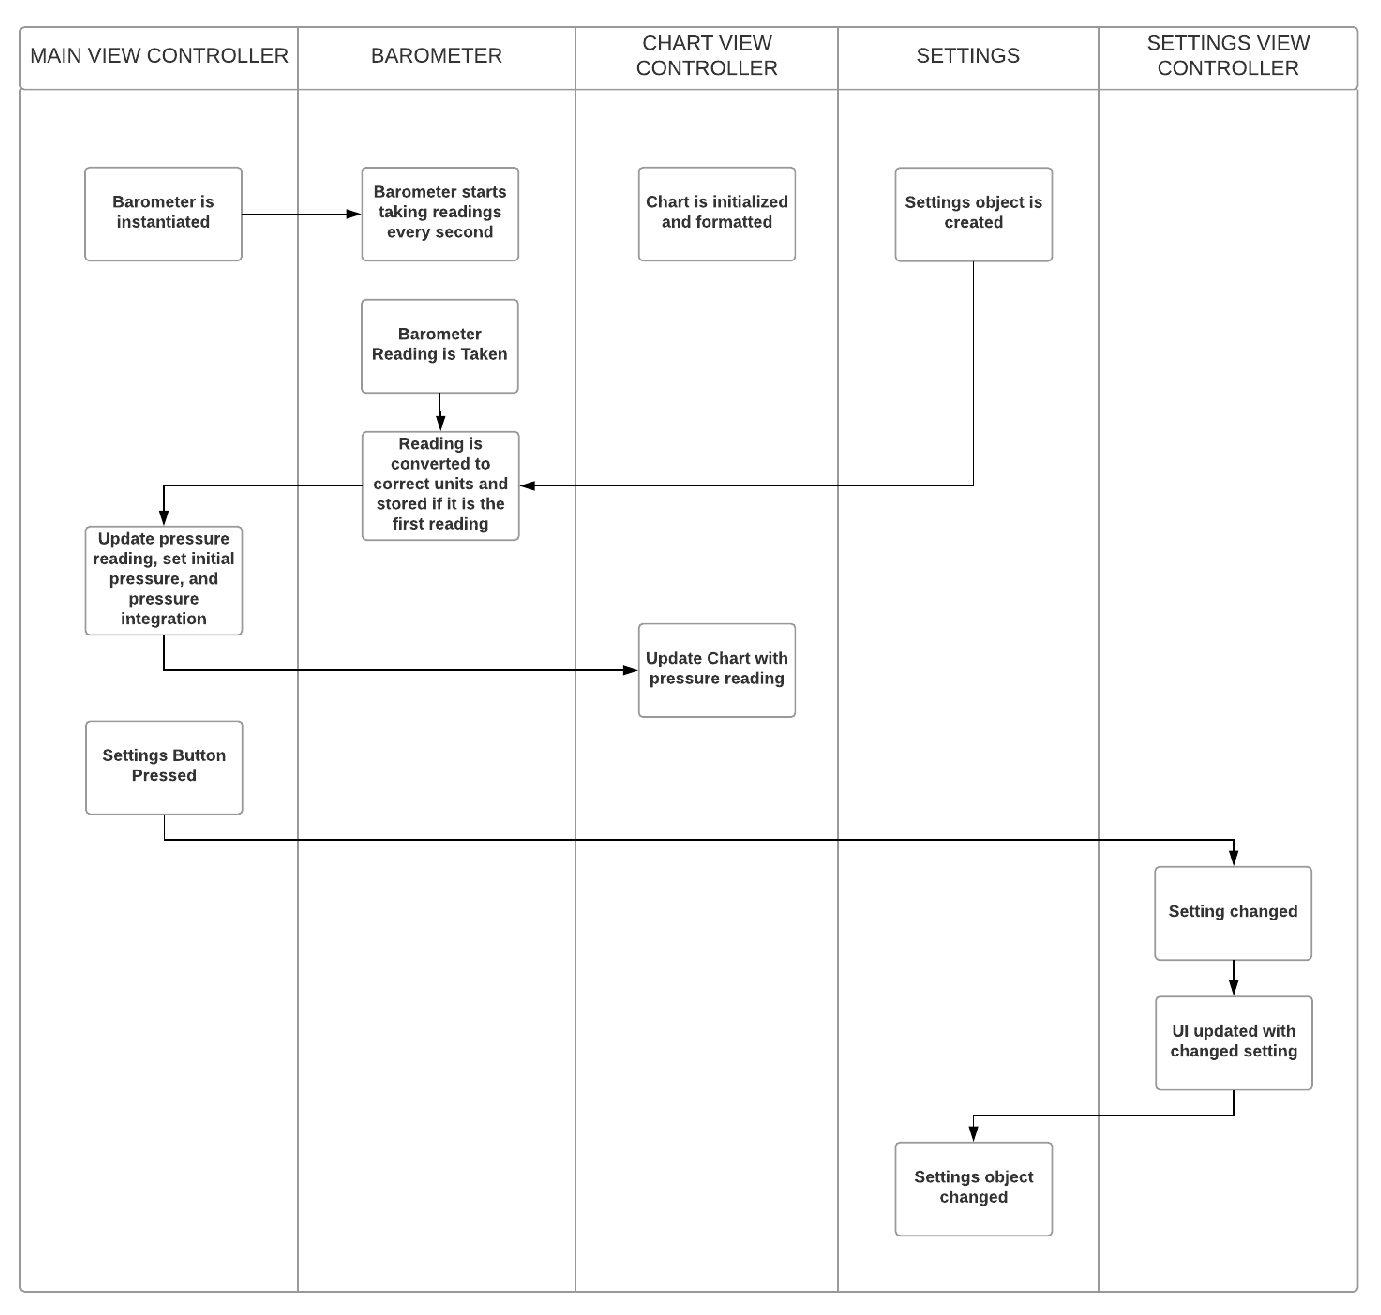
\includegraphics[scale=0.8]{flowchart}

\subsection{How to Run}
To run the project you need to have Xcode installed.
To install the project, fetch the most recent version from github, and run the Build script found in the root folder.
This installs the charts library used to draw the barometer chart.
If Cocoa pods is not already installed on the machine, you may need to run the Build script a second time to successfully install the dependencies.
From there to run the application in a simulator, select iPad Air 2 from the target device dropdown menu.
If you want to run the application on a real device, you need to have an apple developer account.
Just click on the project folder at the top of the hierarchy and change the team to your developer account.

\section{Recommended Technical Resources for Learning More}
% CR
% What web sites were helpful? (Listed in order of helpfulness.)
% What, if any, reference books really helped?
% Were there any people on campus that were really helpful?

\section{Conclusions and Reflections}
% (each team member answers all questions individually)
% What technical information did you learn?
% What non-technical information did you learn?
% What have you learned about project work?
% What have you learned about project management?
% What have you learned about working in teams?
% If you could do it all over, what would you do differently?
% Be honest here -- no B.S.

\subsection{Daniel's Conclusions and Reflections}

\subsection{Nathan's Conclusions and Reflections}

\subsection{Cade's Conclusions and Reflections}
I learned how to use swift coding language. This also taught me how to use xcode as it works well with swift. I learned how to use and navigate through UI view controllers. I learned how to send variables from one view controller to another. I learned how view controllers use or interact with global variables, there can be a global variable for all view controllers or just certain ones. Learned how to use stacks and then even more indefet use views to center objects in view controllers, this helped with organization and adding axis to the the graph. Learned how to lock and orient the screen, this was a problem that took a lot of time to figure out as there wasn't very good documentation on it. The answer was barely longer then a line of code. 
    
I learned how to communicate better, with clients and teammates. Learned about how to set up meetings and sacrificing your time to meet with the client. Time change was a new thing to think about, learned that you need to double check your time and their time so you aren't early to the meeting or late to the meeting.  

    Project work uses a lot more documentation then i had ever realized. I learned that the reason for this is so that you can always go back and look at what was required as it was in written form. I was also very scared of project work thinking that a client would be yelling at us alot and telling us we were doing it wrong or that's not what they wanted a lot. My experience was nothing like that, Don was very polite and worked through us with everything we did. Never got mad at us just told us what we could change and make better. Project work is not to be scary as i thought previously but is more work on paper. 

    I learned that i like the agile style of of project management, working for a few weeks and getting in contact with the client to go over what's been done. I also learned that not everyone schedule can always line up making it hard to have meetings sometimes. When managing a project you need to have everything laid out on paper as well. Using a service like github makes it easy to lay out who needs to do what by when as well. 
    
    I hated working in teams in almost every single project I have ever had except this one. I learned that not everyone will let you down and sometimes you are the person who needs to catch up and do more. This team worked well together and even communicated well, not just well but politely. Even when someone was behind on their work they were not attacked they were reminded and even offered help 
    If i could do it all over again. I would have done even more on the project, i would have asked for help more from my teammates. I would have liked to talk about their parts more in depth so that i understood every single line of code not just some of mine and most of theirs. I would have liked to also have gotten to know my teammates even better than I already did. 

\section{Appendix 1: Essential Code Listings}
% DK
% You don't have to include absolutely everything, but if someone wants to understand your project, there should be enough here to learn from. If you worked within a larger project, something like a patch file might be a good way to go.
\subsection{Barometer.swift}
    \begin{lstlisting}
func startDisplayingPressureData(_ updateFunc:@escaping (Double, Double) -> (),
 _ setInitialPressure:@escaping (Double, Double) -> ()) {
    altimeter.startRelativeAltitudeUpdates(to: OperationQueue.main, withHandler: {
        data, error in
        let kPa = data?.pressure.doubleValue
        let pressure = self.kPa2units(kPa: kPa!)
        let time = Date().timeIntervalSince1970
        if self.initialPressureReading == nil {
            self.initialPressureReading = pressure
            self.initialTime = time
            setInitialPressure(pressure, time)
        }
        if self.updateInitialPressureReading == true {
            setInitialPressure(self.initialPressureReading, self.initialTime)
            self.updateInitialPressureReading = false
        }
        self.pressureReadings.append((pressure, time))
        updateFunc(pressure, time)
    })
}
    \end{lstlisting}

\subsection{Settings.swift}
    \begin{lstlisting}
class Settings: Codable {
    var units = "mmHg"
    var sigFigs = 4
    var orientation = "Right"
    var runningIntegrationInterval = 4
    var slidingScale = false
    var slidingScaleThreshold = 20
    var windowSize = 50
    var pressureBuffer = 58.66
}
\end{lstlisting}

\subsection{MainViewController.swift}
    \begin{lstlisting}
func updateUI(pressure:Double, time:Double) {
    let date = Date(timeIntervalSince1970: time)
    pressureDisplay.text = String(format:"%.\(settings.sigFigs)f", pressure)
    currentTimestamp.text = DateFormatter.localizedString(from: date, dateStyle: .none, timeStyle: .medium)
    currentdPdt = barometer.getDpdt()
    dpdtDisplay.text = String(format:"%.\(settings.sigFigs)f", currentdPdt)
    dtdpDisplay.text = String(format:"%.\(settings.sigFigs)f", barometer.getDtdp())
    chartViewController.updateChart(pressureReading: pressure, time: time)
    updateTRes()
}
    \end{lstlisting}

\subsection{ChartViewController.swift}
    \begin{lstlisting}
func updateChart(pressureReading: Double, time: Double) {
    let newEntry = ChartDataEntry(x: time, y: pressureReading)
    if (currentCount == 0) {
        startTime = time
    }
    if (settings.slidingScale && currentCount <= settings.windowSize) {
        lineChartView.xAxis.axisMinimum = startTime
        lineChartView.xAxis.axisMaximum = Double(settings.windowSize) + startTime
    }
    addDataPoint(newEntry: newEntry)
    updateChartView()
}
    \end{lstlisting}

\subsection{SettingsViewController.swift}
    \begin{lstlisting}
@IBAction func unitPicked(_ sender: Any) {
    let selectedIdx = unitPicker.selectedSegmentIndex
    let selectedUnit = unitPicker.titleForSegment(at: selectedIdx)
    let kpaOfField = Barometer().unit2kPa(pres: Double(minimumPressureField.text!)!)
    chartVC.convertDataPoints(unit: selectedUnit!)
    settings.units = selectedUnit!
    minimumPressureUnit.text = selectedUnit!
    minimumPressureField.text = String(format:"%.3f", Barometer().kPa2units(kPa: kpaOfField))
}
    \end{lstlisting}

\newpage
\bibliographystyle{IEEEtran}
\bibliography{bibliography}

\end{document}
